\documentclass{article}

\usepackage[utf8]{inputenc}
\usepackage[T1]{fontenc}
\usepackage[spanish]{babel}
\usepackage{times}
\usepackage{wrapfig}
\usepackage{lmodern}
\usepackage{mathtools}
\usepackage{graphicx}
\usepackage[utf8]{inputenc}
\usepackage{color}
\usepackage{hyperref}
\usepackage{fancyhdr,lipsum}
%definir los marcos, fondos, numero y demás de los códigos de SQL
\usepackage{listings} 
  \lstset{ frame=Ltb,
          framerule=0pt,
          aboveskip=0.5cm,
          framextopmargin=3pt,
          framexbottommargin=3pt,
          framexleftmargin=0.4cm,
          framesep=0pt,
          rulesep=.4pt,
          backgroundcolor=\color{gray97},
          rulesepcolor=\color{black},
          %
          stringstyle=\ttfamily,
          showstringspaces = false,
          basicstyle=\small\ttfamily,
          commentstyle=\color{gray45},
          keywordstyle=\bfseries,
          %
          numbers=left,
          numbersep=15pt,
          numberstyle=\tiny,
          numberfirstline = false,
          breaklines=true,
  }
\definecolor{gray97}{gray}{.97}
\definecolor{gray75}{gray}{.75}
\definecolor{gray45}{gray}{.45}

% minimizar fragmentado de listados
\lstnewenvironment{listing}[1][]{\lstset{#1}\pagebreak[0]}{\pagebreak[0]}
\lstdefinestyle{consola}{basicstyle=\scriptsize\bf\ttfamily, backgroundcolor=\color{gray75}, }
\lstdefinestyle{C}{language=C,}


\hypersetup{
    colorlinks=true, %set true if you want colored links
    linktoc=all,     %set to all if you want both sections and subsections linked
    linkcolor=blue,  %choose some color if you want links to stand out
}
\urlstyle{same}

\title{PRACTICA TEMA 2}
\author{Antonio Muñoz Cubero}
\date{12 de Noviembre de 2020}

\begin{document}
  \maketitle
    \pagenumbering{gobble}
      \pagestyle{fancy}
  
  \newpage
    \tableofcontents
      \lhead[PRACTICA TEMA 2]{PRACTICA TEMA 2}
        \lfoot[IES Francisco De Los Rios]{IES Francisco De Los Rios}

  \newpage
    \pagenumbering{arabic}
    \section{Enunciado}
    
    Tenemos que copiar  el  código del archivo adjunto, que este caso, muestro en la imagen inferior.
    \begin{itemize}      
      \item Compilar el programa y corregir los errores sintácticos. Incluyendo las librerías que sean necesarias.
      \item Realizar la depuración y posterior ejecución del programa.
      \item Personalizar la configuración del IDE, creando una configuración nueva, llamada \textbf{miconfiguración} para ese proyecto de la siguiente manera: 
      El directorio de trabajo será una carpeta llamada \textit{DirectorioTrabajoED}, que estará situada en el escritorio.
      \item Tras ello, desinstalar los plugins instalados anteriormente.
      \item Actualizar todos los complementos del IDE (si no hay nada que actualizar pon la captura de la pantalla donde se indica).
    \end{itemize}

    \begin{figure}[h]
      \centering
      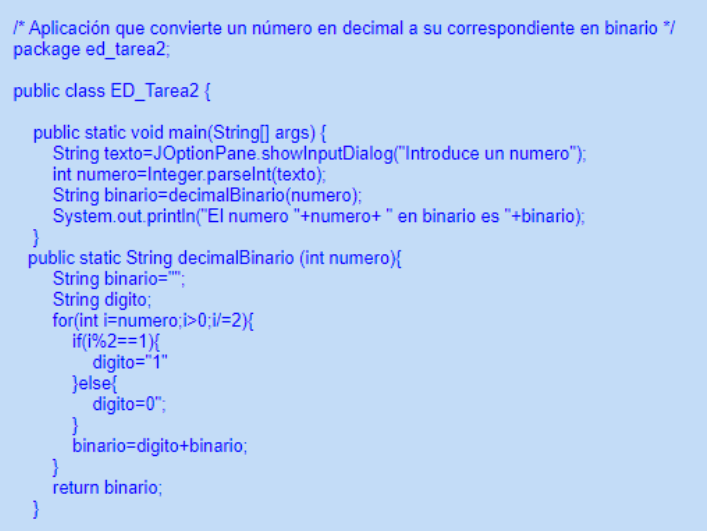
\includegraphics[scale = 0.5]{img/codigo.png}
    \end{figure}
  \newpage
    \section{Primeros pasos}
      \subsection{Creacion del Workspace}
        Lo primero que hacemos al empezar a trabajar en un projecto utilizando, en este caso, el IDE \textit{Eclipse}, es crear nuestro lugar de trabajo o como en el IDE es llamado
        \textbf{"Workspace"}. realizandose de la siguiente manera:
        \begin{figure}[h]
          \centering
          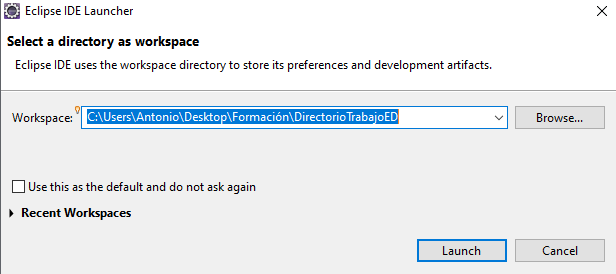
\includegraphics[scale = 0.75]{img/workspace.png}
          \caption{Ventana al inicar Eclipse donde elegimos nuestro workspace.}
        \end{figure}
        Una vez tenemos nuestro espacio de trabajo, ahora procedemos a personalizar nuestro IDE para comenzar a escribir nuestro código.
  \newpage      
    \subsection{Personalización del IDE}
      En mi caso lo primero que haré será modificar las preferencias para que al \textit{"tabular"}, Eclipse interprete que ponga \textbf{2 espacios} y no lo que venga 
      por defecto. Esto es algo de gusto personal y no influye en nada más.\\
      Para cambiar dichas preferencias tenemos que irnos a \textit{Window $\rightarrow$ Java $\rightarrow$ Code Style $\rightarrow$ Formatter}, una vez en \textit{Formatter} le damos a \textit{new}.
      \begin{figure}[h]
        \centering
        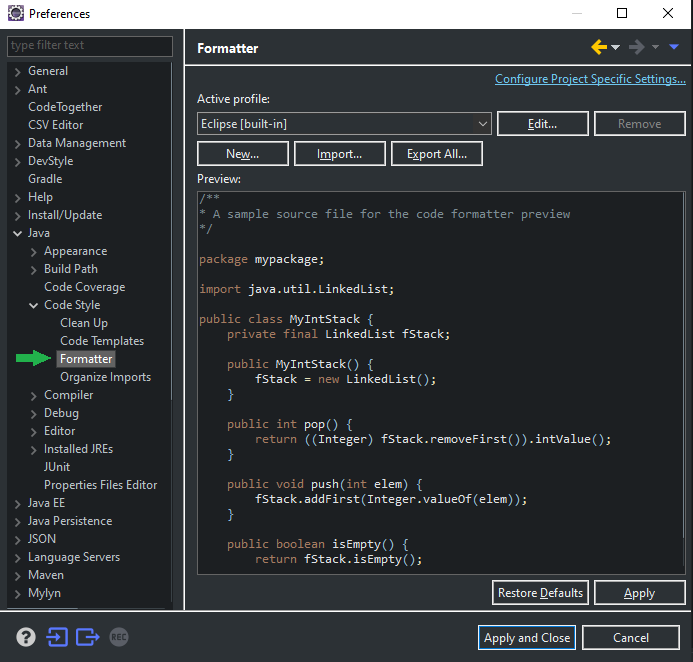
\includegraphics[scale = 0.7]{img/formato.png}
        \caption{Ventena para añadir o editar formatos}
      \end{figure}
  
  \newpage
      Una vez dentro, ponemos nombre a nuestra nueva configuración, en este caso, tal y como dicta esta práctica se llamará \textbf{miconfiguracion}. Además he añadido la siguiente 
      configuración.
      \begin{figure}[h]
        \centering
        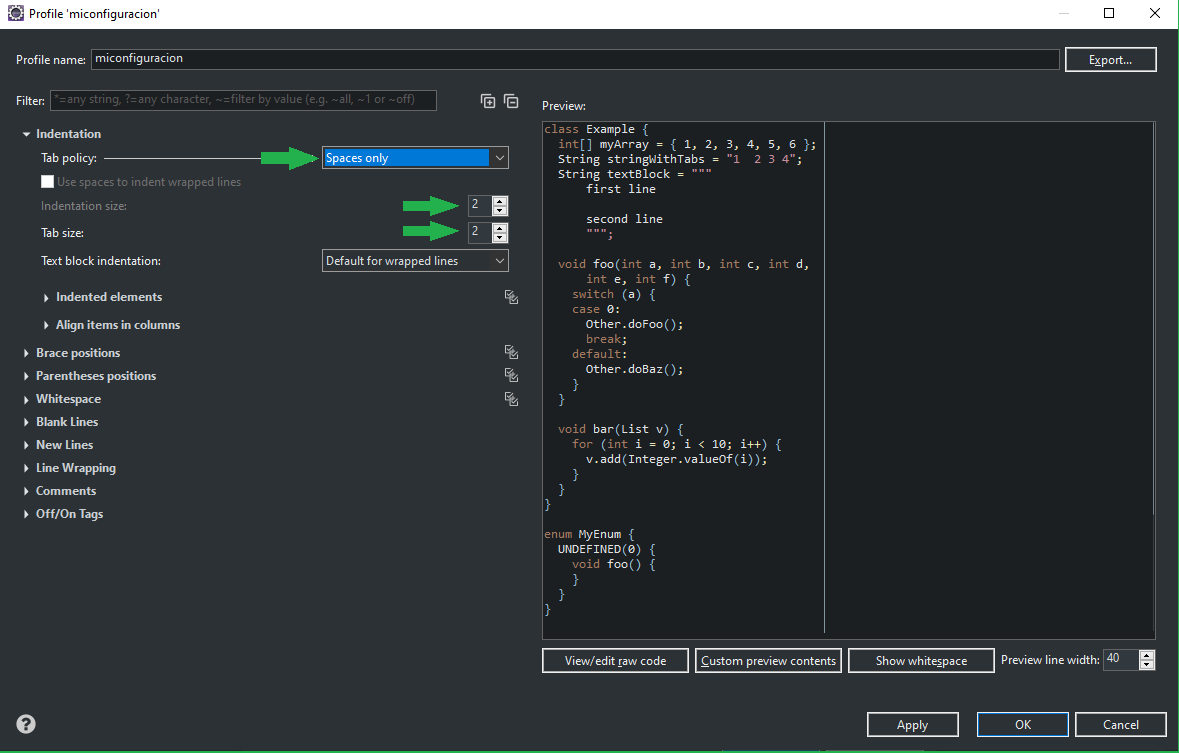
\includegraphics[scale = 0.4]{img/miconfiguracion-profile.png}
        \caption{Preferencias de \textit{miconfiguracion}}
      \end{figure}

      Y hecho esto, ya tendríamos el formato que queremos, además de eso, yo quiero instalar un \textit{"Plugin"} para que Eclipse se vea más bonito.
      Por tanto para ello nos iremos a \textit{Help $\rightarrow$ Marketplace $\rightarrow$ Populars} e instalamos \textbf{Darkest Dark Theme} como vemos en la imagen.
      \begin{figure}[h]
        \centering
        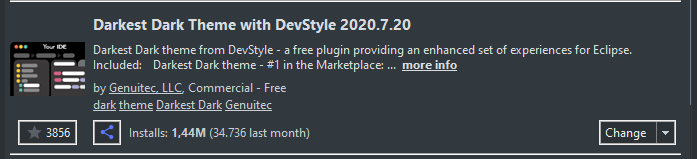
\includegraphics[scale = 0.7]{img/plugin.png}
        \caption{Plugin para un nuevo Theme de Eclipse}
      \end{figure}

  \newpage
    \section{Proyecto}
      \subsection{Creación del Proyecto}
        Una vez tenemos nuestro entorno de trabajo listo a nuestro gusto y con todas las herramientas funcionando a la perfección, pasamos a la creación del proyecto.
        Para ello, seguimos la siguiente ruta una vez tengamos abierto nuestro Workspace como hemos hecho anteriormente, 
        \textit{File $\rightarrow$ New $\rightarrow$ Project}.

        \begin{figure}[h]
          \centering
          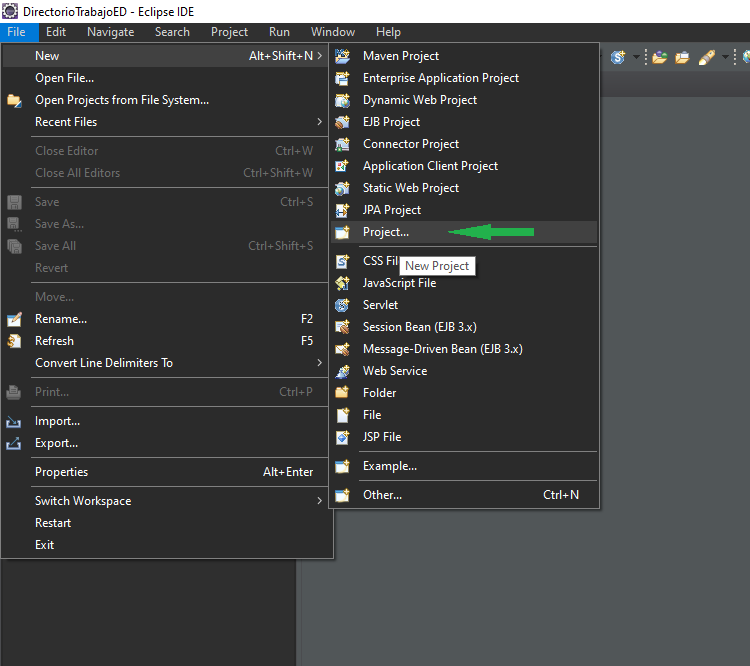
\includegraphics[scale = 0.5]{img/newproject.png}
          \caption{Creación de un nuevo proyecto}
        \end{figure}
        
        Una vez seleccionado \textit{Project} nos aparecera una lista donde deberemos seleccionar \textit{Java $\rightarrow$ Java Project}.

  \newpage
        
        \begin{figure}[h]
          \centering
          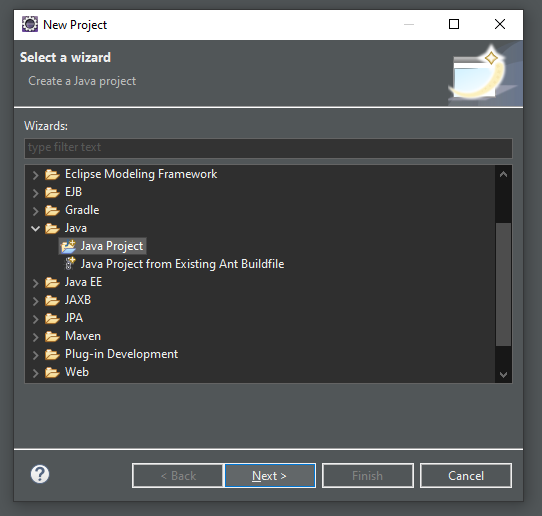
\includegraphics[scale = 0.4]{img/javaproject.png}
          \caption{Distintos formatos de proyectos en Eclipse}
        \end{figure}

        Una vez seleccionado \textit{Java Project} nos aparecerá una ventana de Personalización para nuestro proyecto donde debemos incluir el nombre que le vamos a dar 
        en mi caso \textbf{ED-Tarea2} seleccionar la ubicación por defecto y nuestro \textit{JDK} por defecto
        y pulsar \textit{Finish}.

        \begin{figure}[h]
          \centering
          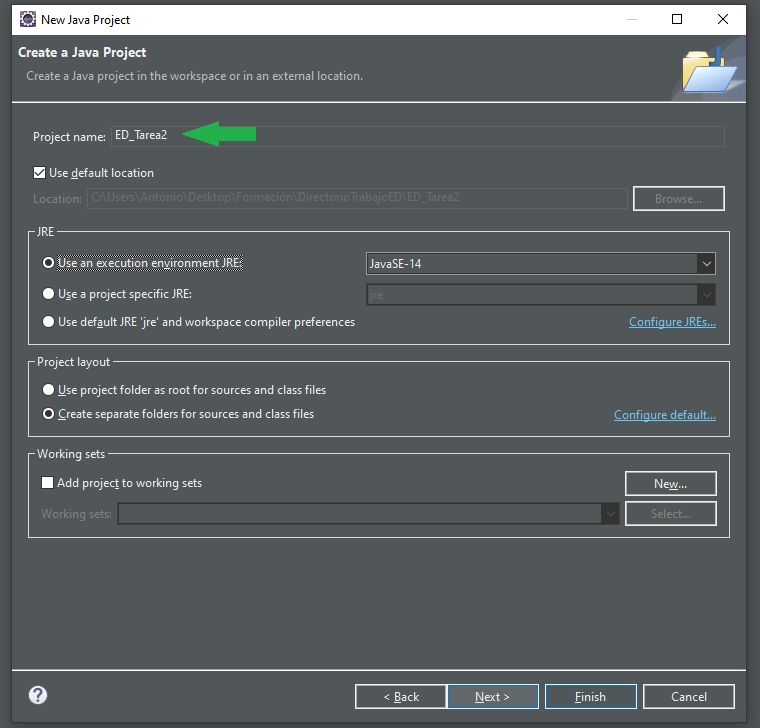
\includegraphics[scale = 0.35]{img/configuration_project.png}
          \caption{Configuracion del proyecto, primera vista.}
        \end{figure}
        
  \newpage
    \subsection{Creación de la Clase}
          Después de haber creado nuestro proyecto, el siguiente paso en la tarea es crear nuestra \textit{Clase} para poder pasar a copiar nuestro código.
          Para ello debemos seguir la siguiente ruta \textit{File $\rightarrow$ New $\rightarrow$ Class}.
          \begin{figure}[h]
            \centering
            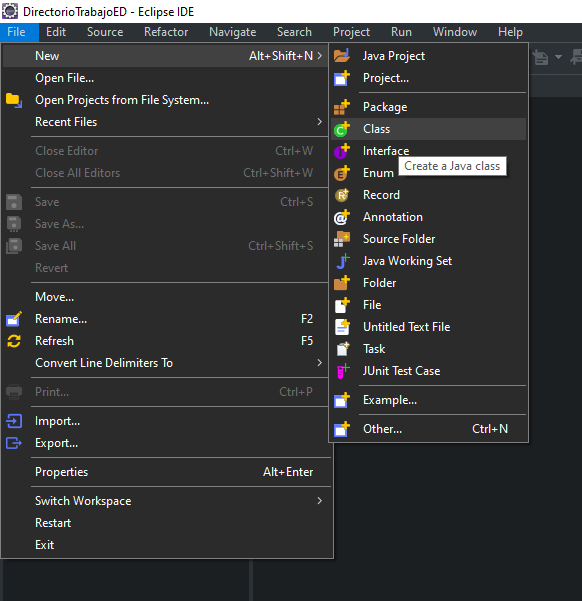
\includegraphics[scale = 0.35]{img/new_class.png}
            \caption{Creación de la clase}
          \end{figure}

          Una vez pulsado el botón de \textit{Class} se nos abrirá una nueva ventana para configurar nuestra Clase Java, donde debemos ingresar el nombre de la clase, si queremos que se 
          incluya en algun \textit{Package}, y los métodos que queramos que cree por defecto, en nuestro caso le diremos que cree un método \textit{main}.
          \begin{figure}[h]
            \centering
            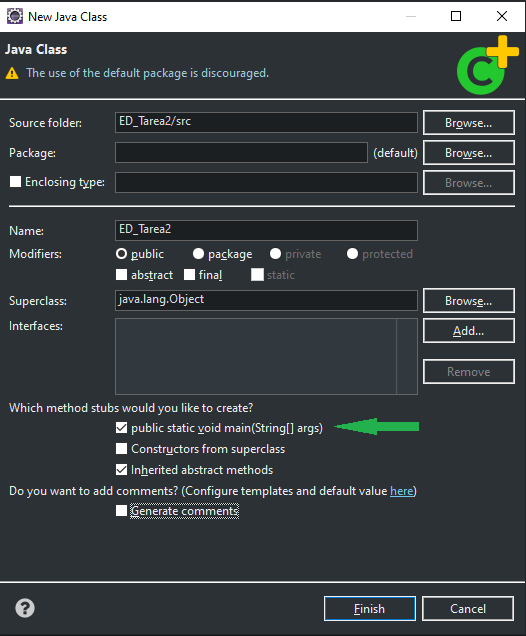
\includegraphics[scale = 0.35]{img/configuration_class.png}
            \caption{Configuración de la clase.}
          \end{figure}



  \newpage
    Una vez creada la clase ahora copiamos el código y seguimos los siguientes pasos.

    \begin{enumerate}
      \item Compilamos para ver errores en el código.
      \item Ejecutamos para ver funcionamiento
      \item Debugeamos para detectar el posible mal funcionamiento
      \item Corregimos el funcionamiento
      \item Compilamos y ejecutamos.
    \end{enumerate}

    El código copiado quedaría tal que así
    \begin{figure}[h]
      \centering
      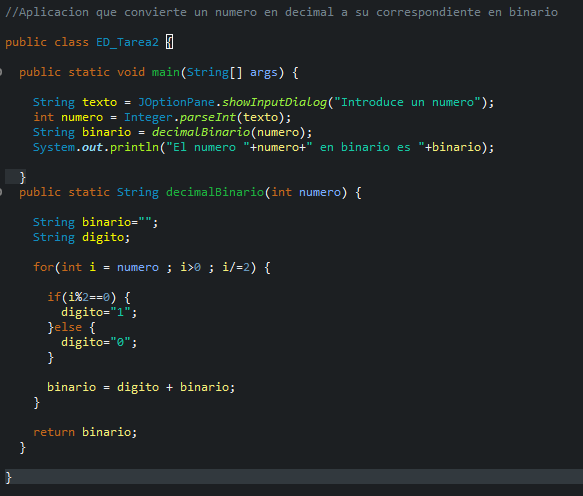
\includegraphics[scale = 0.9]{img/code.png}
      \caption{Código fuente.}
    \end{figure}

  \newpage
    \subsection{Primera compilación}
      Para compilar el programa por primera vez, abrimos nuestra terminal, en mi caso el \textbf{CMD} de Windows, en el directorio donde se encuentre nustro fichero.ç
      Despues de eso, debemos ejecutar la siguiente linea de comandos.
      \begin{listing}[style=consola, numbers=none]
      \$ javac ED_Tarea2.java 
      \end{listing}
      \begin{figure}[h]
        \centering
        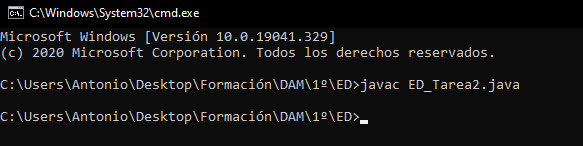
\includegraphics[scale = 0.75]{img/1-compilacion.png}
        \caption{Primera compilación}
      \end{figure}
      Como observamos en la imagen, \textbf{no} se han producido errores, por tanto, procedemos a su ejecución.
      \begin{figure}[h]
        \centering
        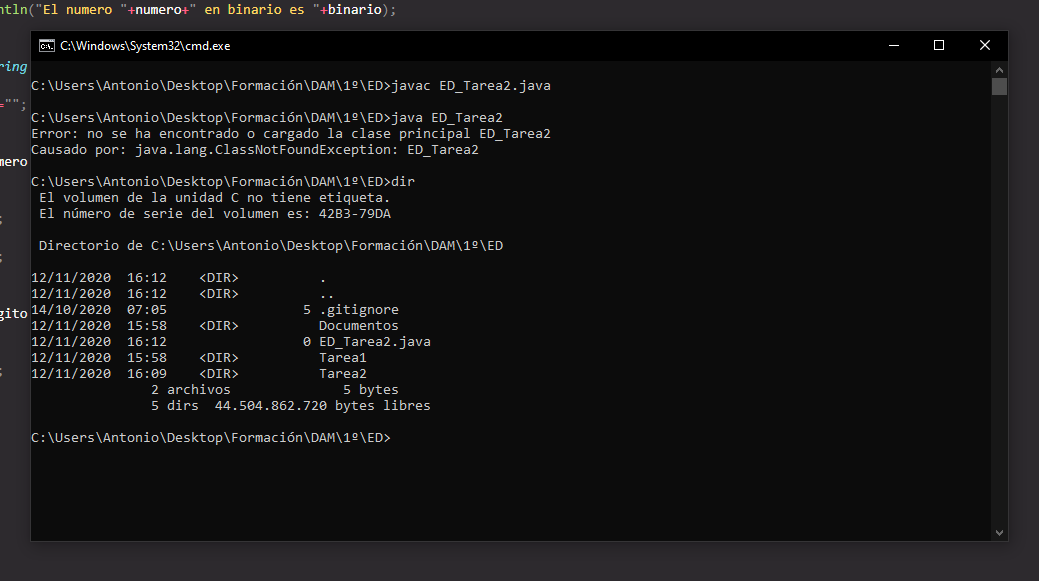
\includegraphics[scale = 0.5]{img/no-class.png}
        \caption{La compilación no crea el .class}
      \end{figure}

  \newpage
    \subsection{Depuración y correción de errores}
      Como hemos visto en la \textit{Figura 10}, cuando hemos compilado, nuestro JDK no crea el .class necesario para la ejecución del programa. Por tanto a la hora de su
      ejecución no podemos llevarla a cabo, pasamos al siguiente paso, la depuración y correción de errores.
      \\\\
      Lo primero que logro identificar en el código de la \textit{Figura 8}, es que no hemos importado las librerías para la ejecución del método 
      \textbf{JOptionPane} y por tanto, esa puede ser una de las causad de dicho error. procedemos a la su implementación añadiendo en las primeras líneas de nuestro código 
      lo siguiente:
      \begin{listing}[style = C]
        import javax.swing.JOptionPane;
      \end{listing}
      Esto hará que importe las librerías necesarias para su uso y no tengamos problemas, después de dicha importación. Procedamos al debugger.

      \begin{figure}[h]
        \centering
        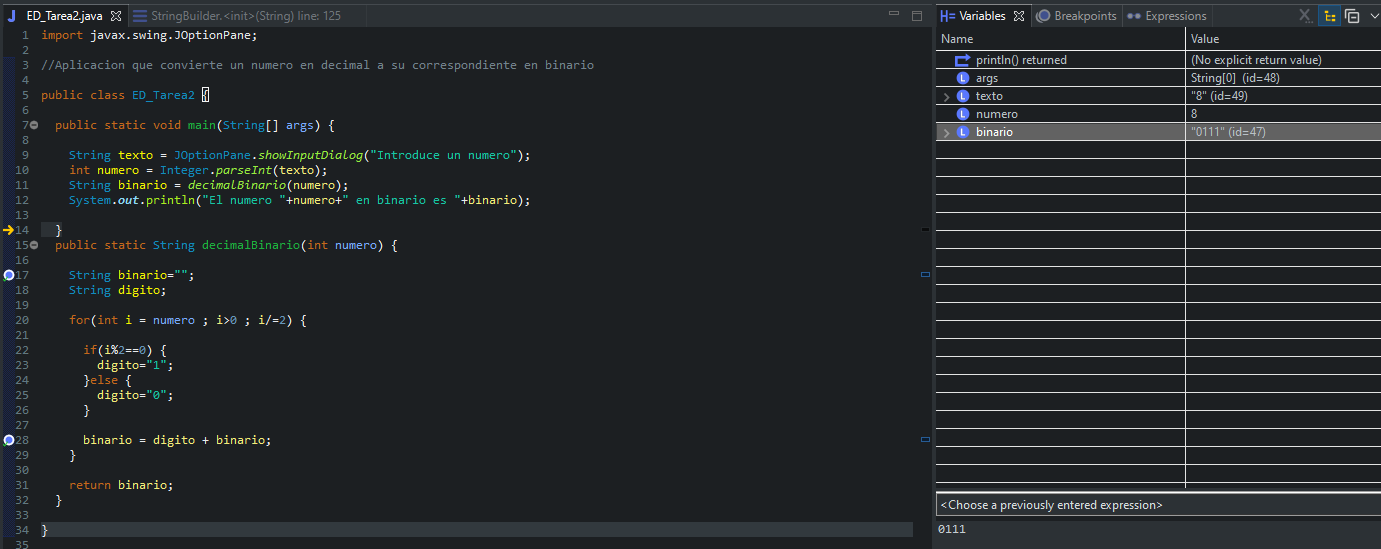
\includegraphics[scale = 0.4]{img/debug.png}
        \caption{Ejecución con el debug}
      \end{figure}

      Obervamos que el binario sale invertido, por tanto, su solución es sencilla, intercambiar las líneas 23 y 25.

  \newpage
    \subsection{Ejecución final}
      Una vez corregido los errores del código, procedemos a compilar el programa para asegurarnos de su buen funcionamiento.
      Ejecutando el mismo comando que anteriormente.
      \begin{listing}[style=consola, numbers=none]
        \$ javac ED_Tarea2.java 
        \end{listing}
      Ahora podemos observar como si nos ha creado nuestro \textbf{.class} correspondiente al archivo \textit{ED-Tarea2.java}
      \begin{figure}[h]
        \centering
        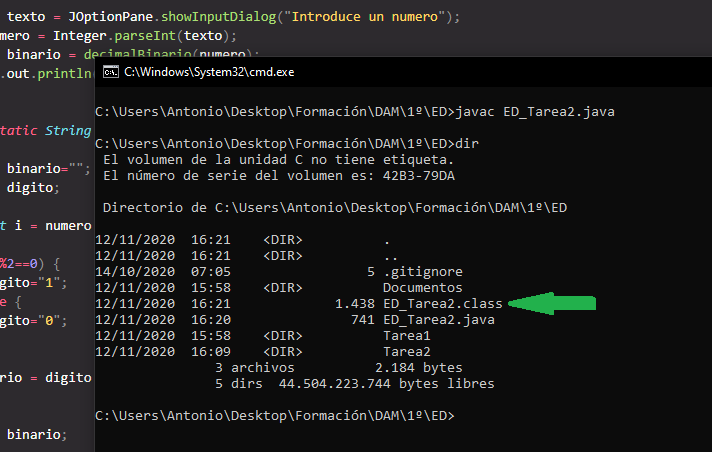
\includegraphics[scale = 0.75]{img/class-creation.png}
        \caption{Creación del .class}
      \end{figure}

      Ahora si podemos proceder a su ejecución, ejecutando el siguiente comando:
      \begin{listing}[style=consola, numbers=none]
        \$ java ED_Tarea2
      \end{listing}

  \newpage
      \begin{figure}[h]
        \centering
        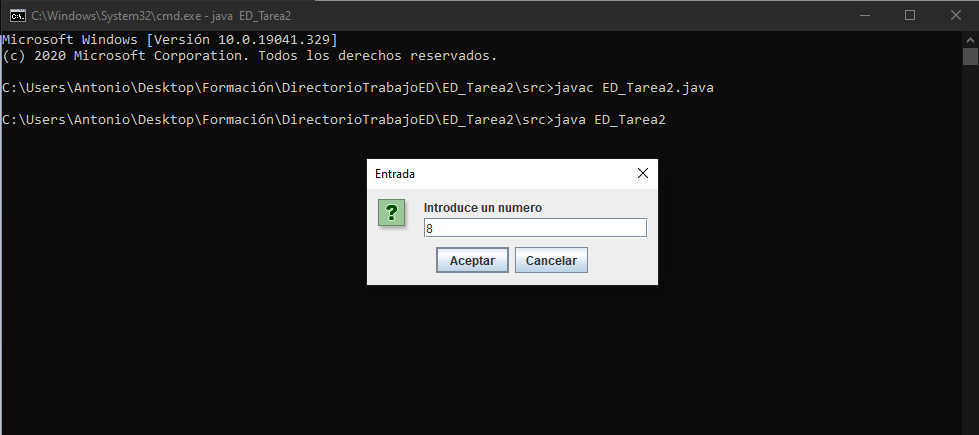
\includegraphics[scale = 0.5]{img/ejecucion.png}
        \caption{Ejecucion ED-Tarea2}
      \end{figure}
      Y obtenemos el siguiente resultado
      \begin{figure}[h]
        \centering
        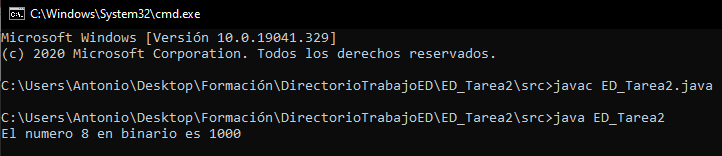
\includegraphics[scale = 0.7]{img/resultado.png}
        \caption{Resultado ED-Tarea2}
      \end{figure}
      
      Ahora nuestro programa funciona correctamente habiendo hecho buen uso del \textbf{Debug} y otras funcionalidades de nustro \textit{IDE Eclipse}.
    
  \newpage
    \section{Desinstalar Plugins}
      Para desinstalar los \textit{plugins} instalados, debemos ir a la siguiente ruta \textit{Help $\rightarrow$ Eclipse Marketplace}
      \begin{figure}[h]
        \centering
        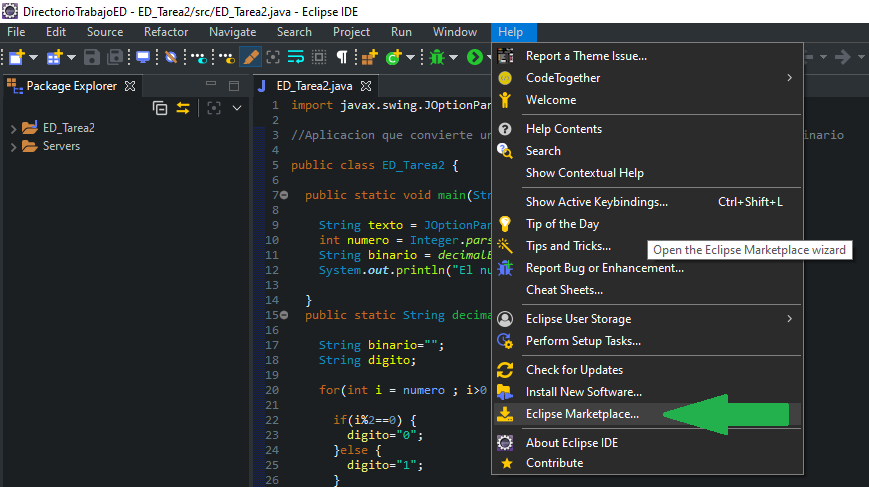
\includegraphics[scale = 0.5]{img/marketplace.png}
        \caption{Ruta a Eclipse Marketplace.}
      \end{figure}
      Una vez dentro nos vamos a la pestaña \textit{Installed} y pulsamos en desinstalar en el plugin que deseemos desinstalar de nuestro IDE.
      \begin{figure}[h]
        \centering
        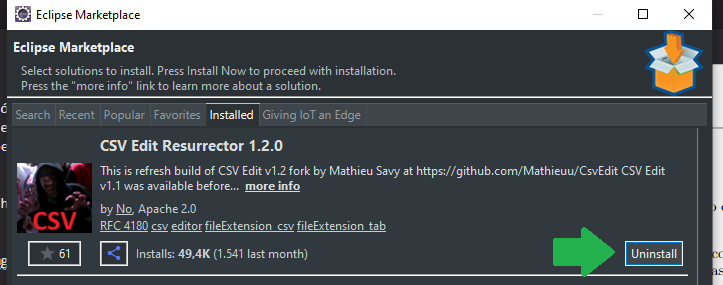
\includegraphics[scale = 0.5]{img/unistall.png}
        \caption{Desinstalar un plugin.}
      \end{figure}

  \newpage
    \section{Actualizar complementos}
      Para actualizar los componentes de nuestro IDE, debemos acceder a la siguiente ruta \textit{Help $\rightarrow$ Check for Updates}
      \begin{figure}[h]
        \centering
        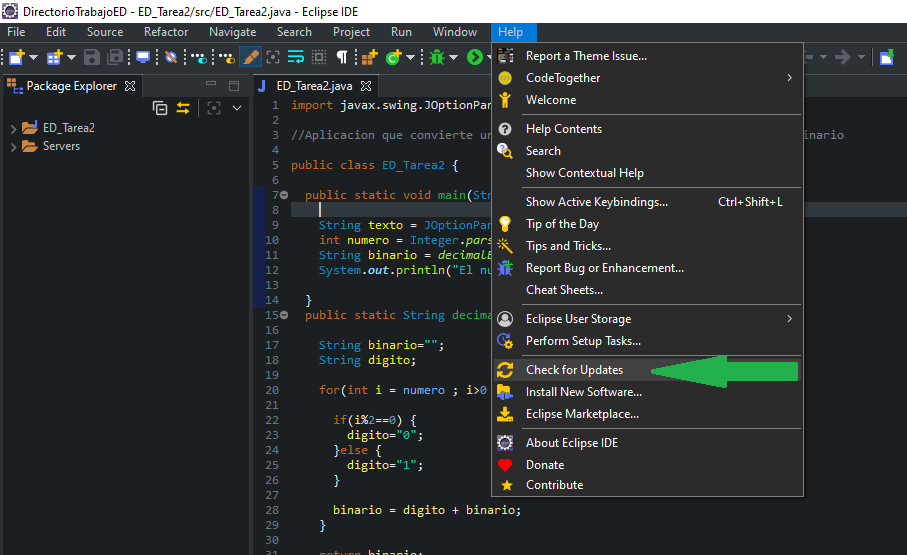
\includegraphics[scale = 0.4]{img/update.png}
        \caption{Ruta para actualizar componentes}
      \end{figure}
      Acto seguido tendremos que esperar un poco mientras comprueba los paquetes que disponen de actualización. Una vez el IDE lo compruebe nos aparecerá
      una ventana donde muestra todos los paquetes que podemos actualizar, debemos pulsar en \textit{Next}
      \begin{figure}[h]
        \centering
        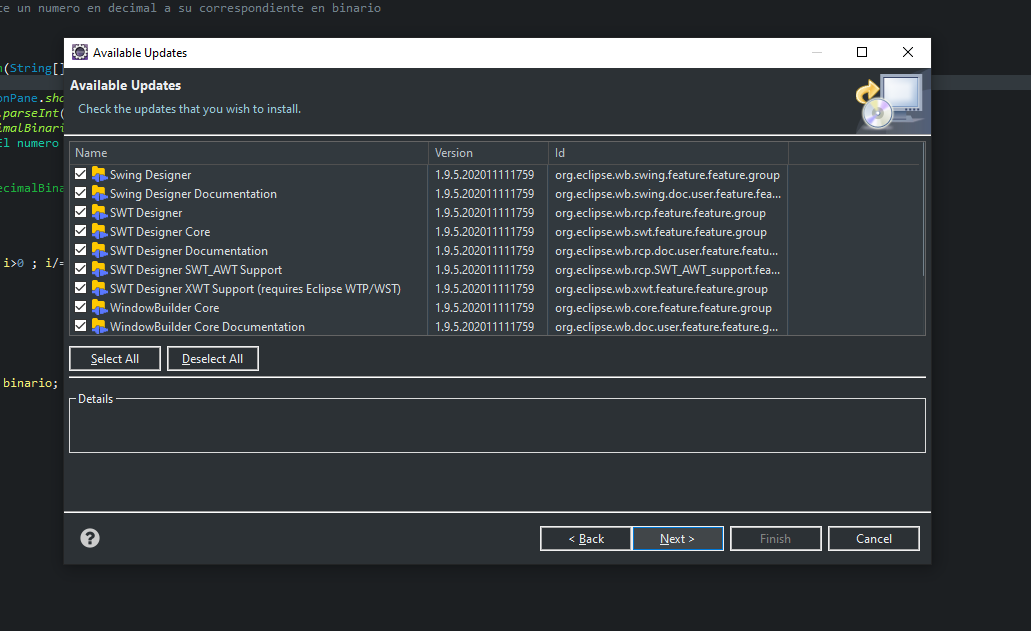
\includegraphics[scale = 0.3]{img/update-3.png}
        \caption{Actualizar componentes.}
      \end{figure}
      Después de esa ventana, aceptaríamos los términos de uso y una vez el programa termine de actualizar todos los paquetes nos pedirá que reiniciemos \textit{Eclipse}.
      Una vez reiniciado, ya tendríamos nuestro paquetes actualizados.
  \newpage
    \section{Índice de Figuras}
    \listoffigures


\end{document}